\documentclass[]{ximera}
%handout:  for handout version with no solutions or instructor notes
%handout,instructornotes:  for instructor version with just problems and notes, no solutions
%noinstructornotes:  shows only problem and solutions

%% handout
%% space
%% newpage
%% numbers
%% nooutcomes

%I added the commands here so that I would't have to keep looking them up
%\newcommand{\RR}{\mathbb R}
%\renewcommand{\d}{\,d}
%\newcommand{\dd}[2][]{\frac{d #1}{d #2}}
%\renewcommand{\l}{\ell}
%\newcommand{\ddx}{\frac{d}{dx}}
%\everymath{\displaystyle}
%\newcommand{\dfn}{\textbf}
%\newcommand{\eval}[1]{\bigg[ #1 \bigg]}

%\begin{image}
%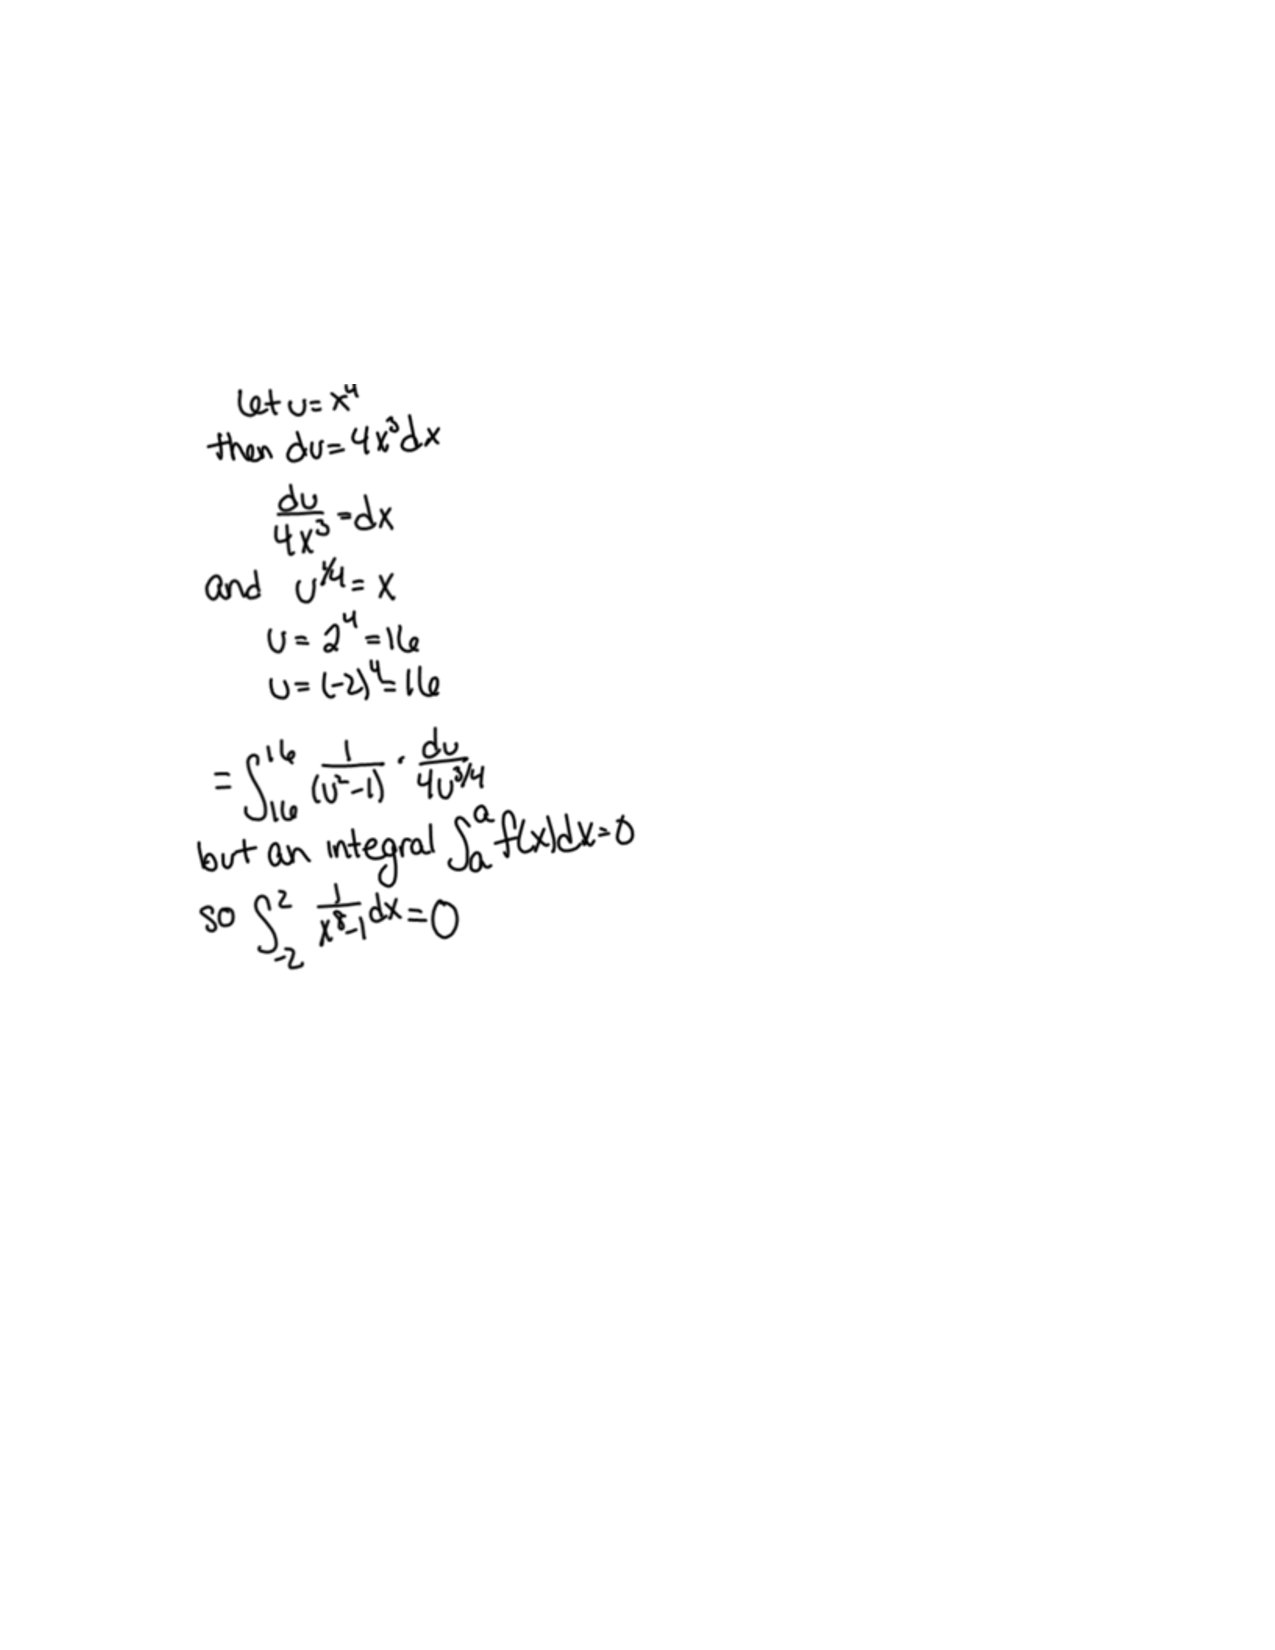
\includegraphics[trim= 170 420 250 180]{Figure1.pdf}
%\end{image}

%add a ``.'' below when used in a specific directory.
\newcommand{\RR}{\mathbb R}
\renewcommand{\d}{\,d}
\newcommand{\dd}[2][]{\frac{d #1}{d #2}}
\renewcommand{\l}{\ell}
\newcommand{\ddx}{\frac{d}{dx}}
\newcommand{\dfn}{\textbf}
\newcommand{\eval}[1]{\bigg[ #1 \bigg]}

\usepackage{multicol}

\renewenvironment{freeResponse}{
\ifhandout\setbox0\vbox\bgroup\else
\begin{trivlist}\item[\hskip \labelsep\bfseries Solution:\hspace{2ex}]
\fi}
{\ifhandout\egroup\else
\end{trivlist}
\fi} %% we can turn off input when making a master document

\title{Alternating series}  

\begin{document}
\begin{abstract}		\end{abstract}
\maketitle



\begin{comment}
\section{Warm up:}

	\begin{freeResponse}
	
	\end{freeResponse}
	
\begin{instructorNotes}

\end{instructorNotes}
\end{comment}







\section{Group work:}



%problem 1
\begin{problem}
Determine if the following series absolutely converge, conditionally converge, or diverge.
	\begin{multicols}{3}
	\begin{enumerate}
	
	\item  $\sum_{n=0}^\infty \frac{(-1)^n}{n+3}$
	
	\item  $\sum_{n=1}^\infty \frac{(-1)^n (n+1)^n}{(2n)^n}$
	
	\item  $\sum_{n=1}^\infty (-1)^{n+1} n^2 e^{\frac{-n^3}{3}}$
	
	\item  $\sum_{n=0}^\infty \frac{(-1)^n \cdot 5}{3^n + 3^{-n}}$
	
	\item  $\sum_{n=4}^\infty \frac{(-2)^n}{n}$
	
	\end{enumerate}
	\end{multicols}
	
	\begin{freeResponse}
	
	\begin{enumerate}
	
	\item
	
	\item
	
	\item
	
	\item
	
	\item
	
	\end{enumerate}
	
	\end{freeResponse}
	
\end{problem}

\begin{instructorNotes}
These problems use a mix of tests.  
One of the main goals is for students to get practice determining which test to use.
	\begin{enumerate}
	\item  Limit Comparison Test with the harmonic series
	\item  Root Test
	\item  Integral Test
	\item  Limit Comparison Test
	\item  Divergence Test.  
	Be sure to talk about ``pulling out the $2$'' to get an alternating series in standard form.  
	Talk about how the Alternating Series Test and the Divergence Test will take care of conditional convergence for most (but not all) alternating series that they will see.
	\end{enumerate}
\end{instructorNotes}







%problem 2
\begin{problem}
\begin{enumerate}

\item  Find an upper bound for how close $\sum_{k=0}^4 \frac{(-1)^k k}{4^k}$ is to the value of $\sum_{k=0}^\infty \frac{(-1)^k k}{4^k}$.

\item  How many terms are needed to estimate $\sum_{n=1}^\infty \frac{(-1)^n \ln n}{n!}$ to within $10^{-4}$?

\end{enumerate}
	\begin{freeResponse}
	\begin{enumerate}

	\item

	\item

	\end{enumerate}
	\end{freeResponse}
		
\end{problem}

\begin{instructorNotes}
Split (a) and (b) among the groups.
\end{instructorNotes}







\begin{comment}
%problem 3
\begin{problem}

	\begin{freeResponse}
	
	\end{freeResponse}

\end{problem}

\begin{instructorNotes}

\end{instructorNotes}
\end{comment}
















	
	
	
	
	
	
	
	
	

	










								
				
				
	














\end{document} 


















